\Chapter{}

\chapter{RESULTADOS}

    \section{Evaluación de la armonización de imágenes MSS y TM}
        \subsection{Corrección geométrica y alineación espacial}
            La aplicación de técnicas avanzadas de corrección geométrica y alineación espacial a las imágenes MSS resultó en una mejora significativa en la precisión de su superposición con las imágenes TM. Utilizando el método LightGlue para el emparejamiento de características, se logró una reducción notable en el error de colocación, pasando de un RMSE inicial de 52.6523 a un RMSE de 0.987. Este resultado subraya la efectividad de las correcciones a nivel de píxel y subpíxel en la alineación de las imágenes, permitiendo una base sólida para la posterior armonización espectral.

            \begin{figure}[H] 
                \caption{\doublespacing \\ \textit{Comparativa de alineación: imágenes MSS, TM y MSS corregida.}} 
                \centering
                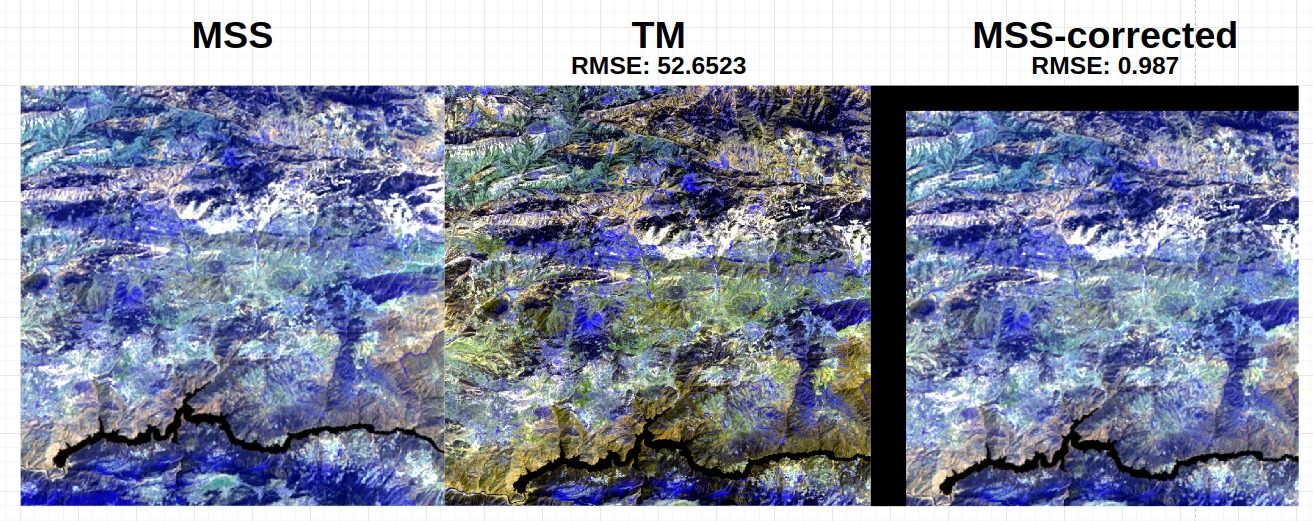
\includegraphics[width=1\linewidth]{2_CAPITULO0/IMG/tm_mss_rmse.png}
                \begin{justify}
                    \textit{Nota.} El contraste entre la imagen MSS original y la corregida resalta con una reducción significativa del error RMSE, evidenciando la eficacia de las correcciones a nivel de píxel y subpíxel para lograr una alineación casi perfecta.
                \end{justify}                    
                \label{tm_mss_rmse}
            \end{figure}

        \subsection{Calidad de la armonización espectral y espacial}
            La implementación del modelo SWINIR - MSS2TM GAN mostró una capacidad excepcional para armonizar las bandas espectrales de las imágenes MSS con las correspondientes imágenes TM. 

            \begin{figure}[H] 
                \caption{\doublespacing \\ \textit{Generación de bandas NIR-R-G armonizadas de MSS hacia TM.}} 
                \centering
                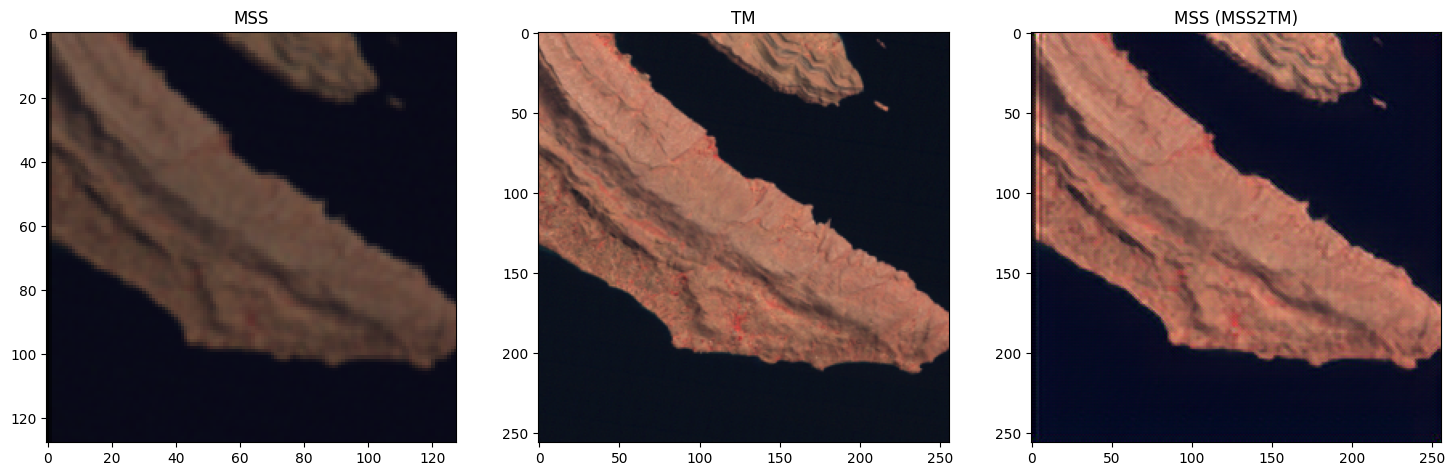
\includegraphics[width=1\linewidth]{2_CAPITULO5/IMG/espectral.png}
                \begin{justify}
                    \textit{Nota.} Comparación entre imágenes MSS, TM y MSS corregida usando el modelo SWINIR - MSS2TM. La imagen MSS original se muestra a la izquierda, la imagen TM original está en el centro, y la imagen MSS corregida se encuentra a la derecha, destacando la mejora en la armonización espectral.
                \end{justify}                    
                \label{armonizacion}
            \end{figure}
            
            \begin{figure}[H] 
                \caption{\doublespacing \\ \textit{Comparación de imágenes MSS antes y después de la mejora en resolución.}} 
                \centering
                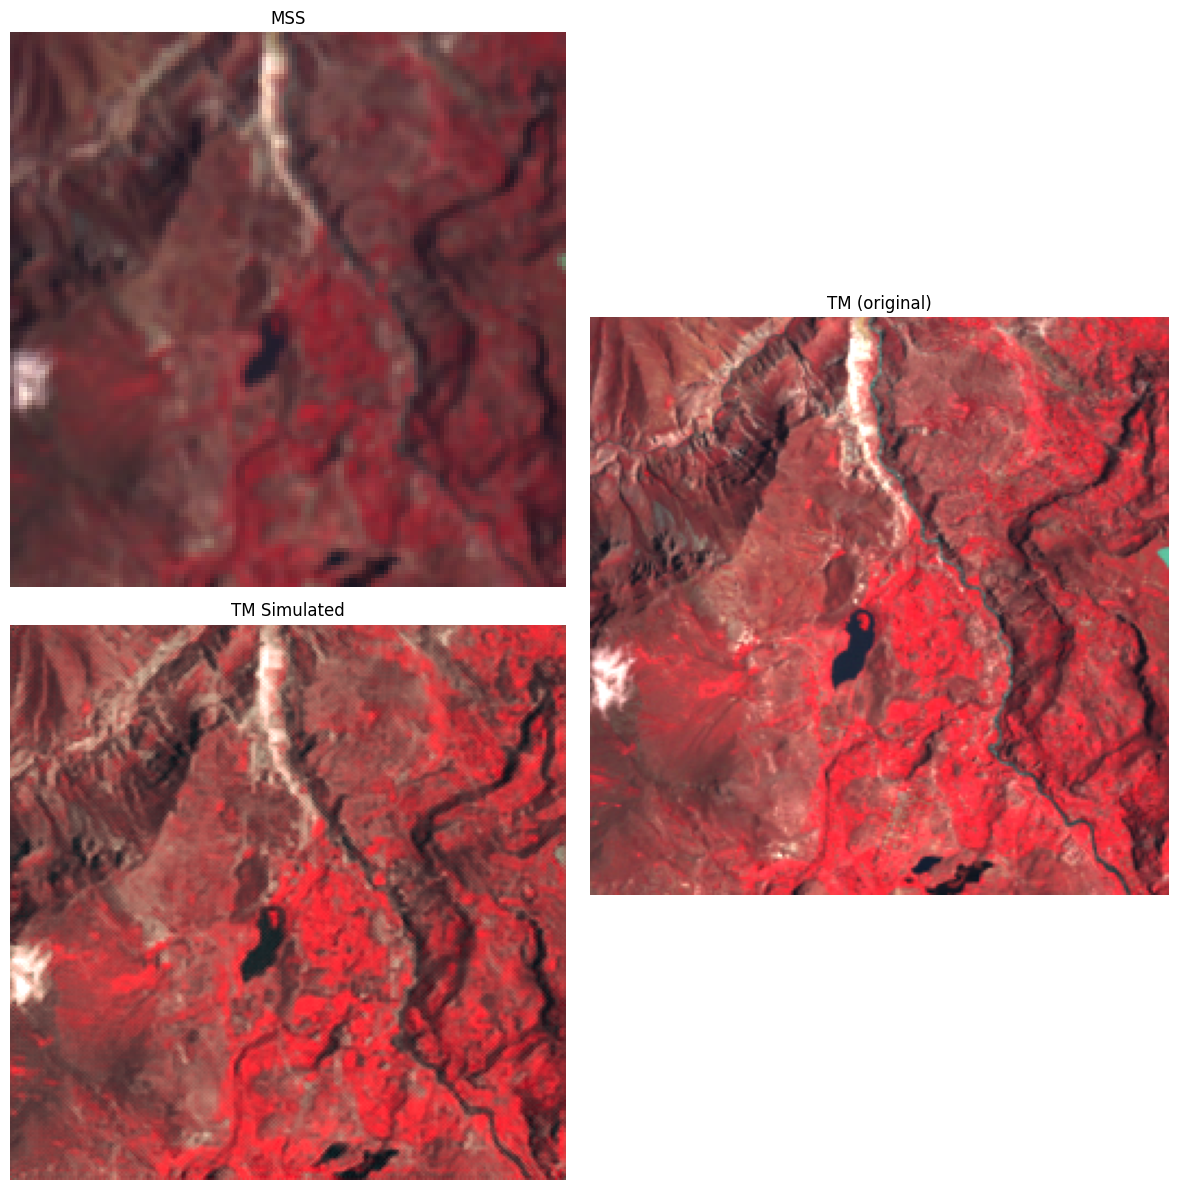
\includegraphics[width=0.8\linewidth]{2_CAPITULO5/IMG/espectral2.png}
                \begin{justify}
                    \textit{Nota.} Comparación de la resolución de imágenes MSS y TM. La imagen MSS original se muestra en la parte superior izquierda, la imagen TM simulada está en la parte inferior izquierda, y la imagen TM original se presenta a la derecha, demostrando la mejora en la resolución de la imagen MSS.
                \end{justify}                    
                \label{armonizacion2}
            \end{figure}
            


        \subsection{Generación de bandas virtuales}
            La creación de bandas virtuales para complementar las imágenes MSS con bandas no originalmente presentes demostró ser altamente efectiva. El modelo de Perceptrón Multicapa (MLP) empleado para predecir estas bandas adicionales alcanzó una alta precisión de predicción, reflejada en un bajo error medio absoluto (MAE). Esta técnica permite mejorar significativamente la calidad de las imágenes MSS, haciéndolas comparables a las imágenes TM en términos de resolución espectral.

            

            \begin{figure}[H] 
                \caption{\doublespacing \\ \textit{Comparación de imágenes Landsat MSS y TM.}} 
                \centering
                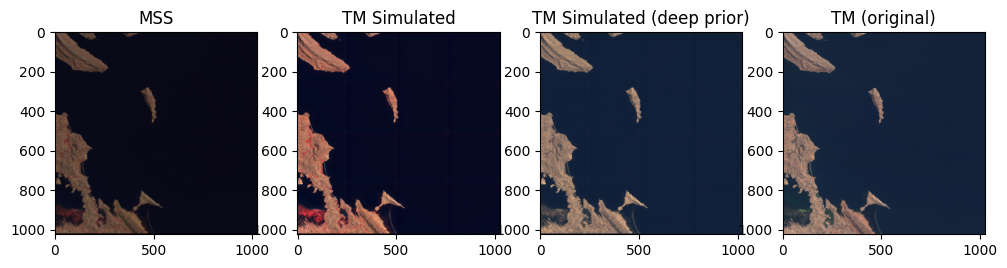
\includegraphics[width=1\linewidth]{2_CAPITULO5/IMG/bandas.png}
                \begin{justify}
                    \textit{Nota.} Visualización del avance en generación de bandas virtuales MSS, mostrando la eficacia del modelo MLP en la precisión espectral frente a imágenes TM originales.
                \end{justify}                    
                \label{bandas}
            \end{figure}

            \begin{figure}[H] 
                \caption{\doublespacing \\ \textit{Comparación de alineación y generación de bandas virtuales.}} 
                \centering
                \includegraphics[width=1\linewidth]{2_CAPITULO5/IMG/comparasion.png}
                \begin{justify}
                    \textit{Nota.} Comparativa de imágenes MSS original, TM simulada con 3 bandas, TM simulada con 7 bandas y TM original, mostrando mejoras en la precisión espectral con modelos avanzados como SWINIR y MLP.
                \end{justify}                    
                \label{bandas2}
            \end{figure}

            La mejora en la resolución es evidente al comparar la imagen MSS original con la imagen TM simulada. Esta mejora permite una mejor interpretación y análisis de los datos históricos de Landsat MSS.

        \subsection{Evaluación de la armonización de imágenes}

            \subsubsection{Índices espectrales} 

                Para evaluar la efectividad de la armonización de imágenes MSS y TM, se calcularon varios índices espectrales tanto para las imágenes originales como para las imágenes simuladas. Los índices utilizados incluyen el Índice de Vegetación de Diferencia Normalizada (NDVI), el Índice de Diferencia Normalizada de Agua (NDWI) y el Índice de Diferencia Normalizada de Nieve (NDSI).

                \paragraph{Índice de vegetación de diferencia normalizada (NDVI)}

                    El NDVI es una métrica importante para el análisis de la vegetación. Se calcula usando las bandas roja (Red) y del infrarrojo cercano (NIR) de la siguiente manera:

                    \begin{equation}
                        NDVI = \frac{(NIR - Red)}{(NIR + Red)}
                    \end{equation}

                    \begin{figure}[H] 
                        \caption{\doublespacing \\ \textit{Comparación de NDVI entre imágenes originales y simuladas.}} 
                        \centering
                        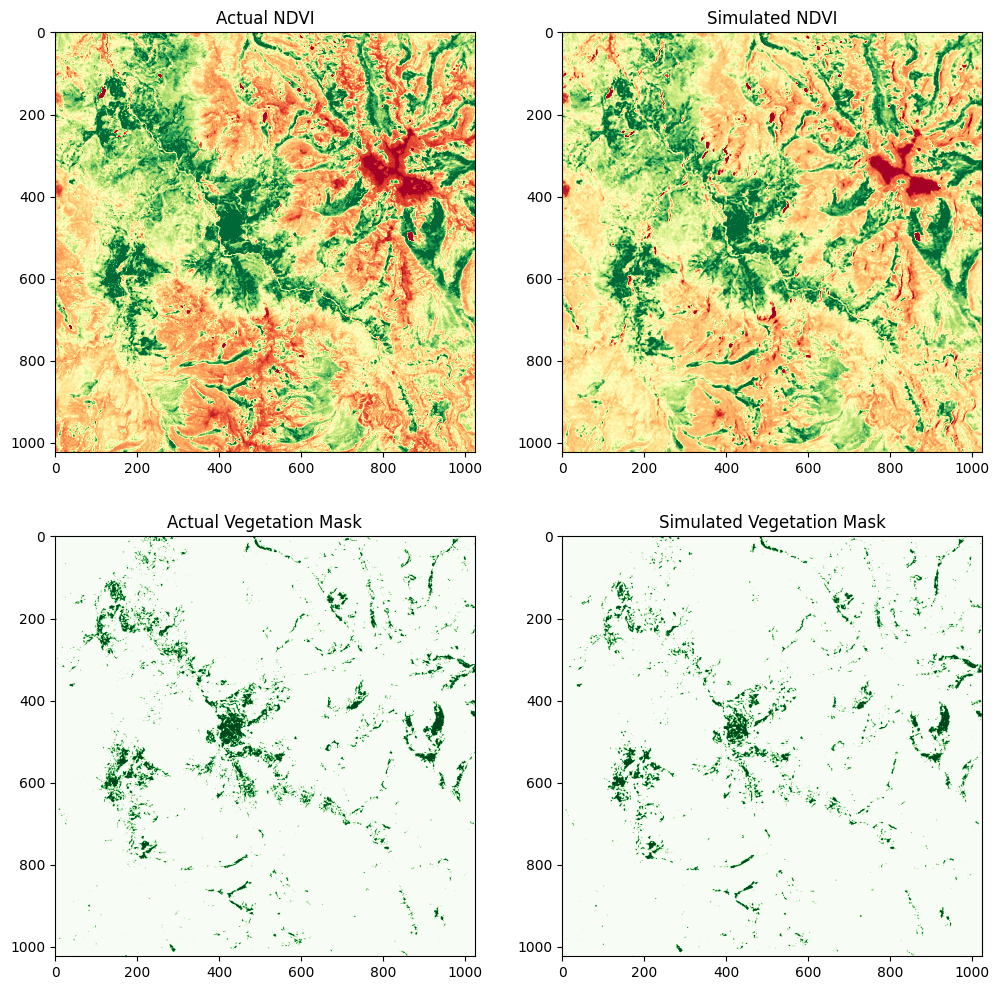
\includegraphics[width=1\linewidth]{2_CAPITULO5/IMG/ndvi2.png}
                        \begin{justify}
                            \textit{Nota.} La comparación de NDVI muestra cómo la vegetación es representada en las imágenes originales y simuladas, destacando la efectividad de la armonización espectral en la detección precisa de la vegetación.
                        \end{justify}                    
                        \label{ndvi2}
                    \end{figure}
        

                \paragraph{Índice de diferencia normalizada de agua (NDWI)}
                    El NDWI es útil para la detección de cuerpos de agua y se calcula usando las bandas verde (Green) y del infrarrojo cercano (NIR):

                    \begin{equation}
                        NDWI = \frac{\text{Green} - \text{NIR}}{\text{Green} + \text{NIR}}
                    \end{equation}

                    \begin{figure}[H] 
                        \caption{\doublespacing \\ \textit{Comparación de NDWI entre imágenes originales y simuladas.}} 
                        \centering
                        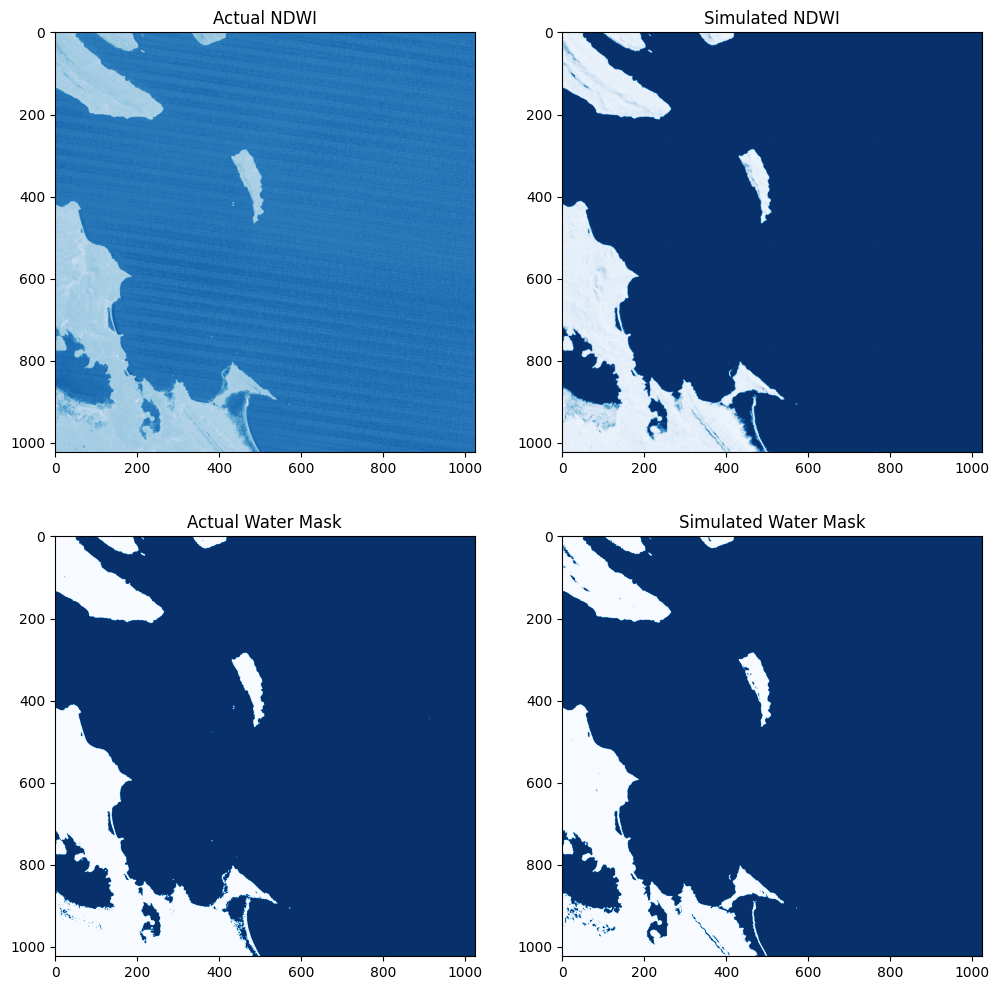
\includegraphics[width=1\linewidth]{2_CAPITULO5/IMG/ndwi.png}
                        \begin{justify}
                            \textit{Nota.} La comparación de NDWI muestra que el modelo detecta cuerpos de agua con mayor precisión en las imágenes simuladas, corrigiendo posibles errores en la banda verde de las imágenes actuales y mejorando la detección a pesar de las imperfecciones originales.
                        \end{justify}                    
                        \label{ndwi}
                    \end{figure}

                \paragraph{Índice de diferencia normalizada de nieve (NDSI)}
                    El NDSI es útil para la detección de nieve y se calcula usando las bandas verde (Green) y del infrarrojo de onda corta (SWIR):

                    \begin{equation}
                        NDSI = \frac{(Green - SWIR)}{(Green + SWIR)}
                    \end{equation}

                    \begin{figure}[H] 
                        \caption{\doublespacing \\ \textit{Comparación de NDSI entre imágenes originales y simuladas.}} 
                        \centering
                        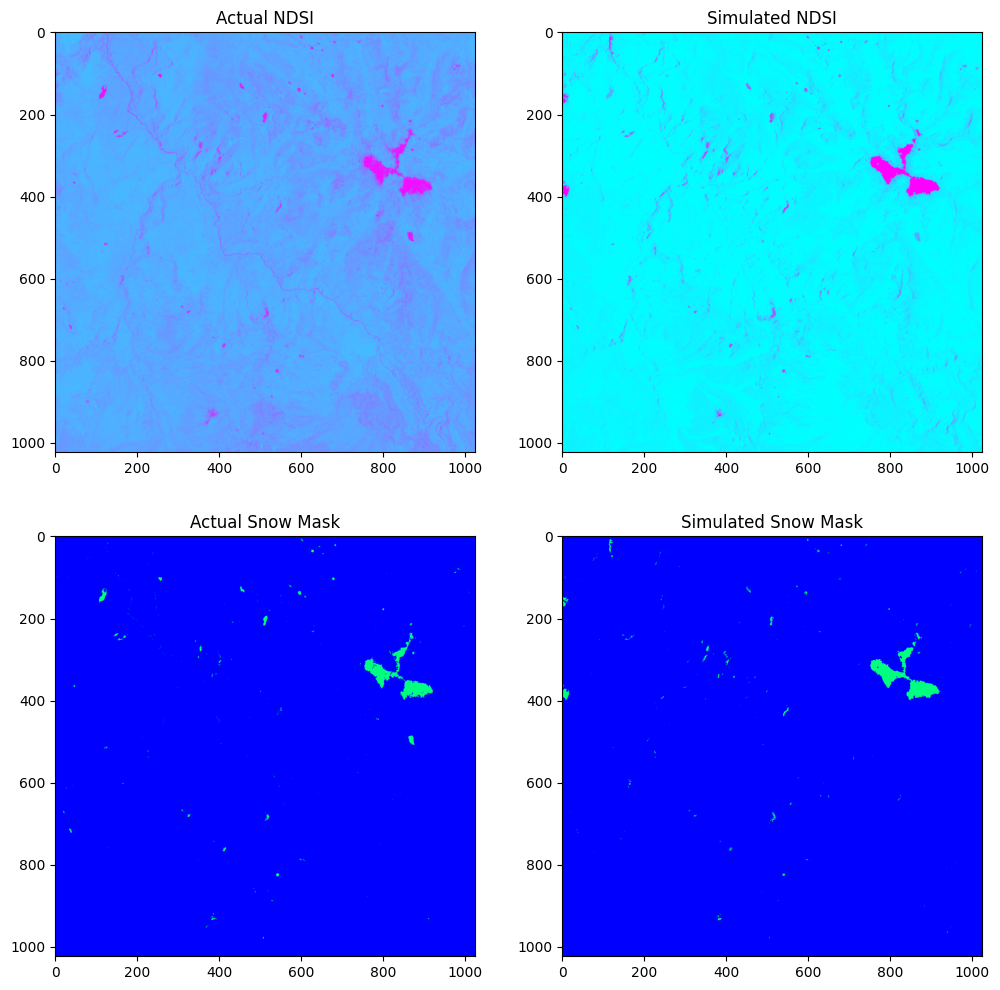
\includegraphics[width=1\linewidth]{2_CAPITULO5/IMG/ndsi2.png}
                        \begin{justify}
                            \textit{Nota.} La comparación de NDSI evidencia la capacidad del modelo para detectar áreas nevadas con precisión en las imágenes simuladas en comparación con las originales.
                        \end{justify}                    
                        \label{ndsi2}
                    \end{figure}
        
    \section{Análisis estadístico de los resultados}
        \subsection{Contexto y metodología de Validación}

            \begin{figure}[H] 
                \caption{\doublespacing \\ \textit{Áreas de validación en Perú.}} 
                \centering
                \includegraphics[width=0.8\linewidth]{2_CAPITULO5/IMG/imagenes_peru.png}
                \label{imagenes_peru}
                \begin{justify}
                    \textit{Nota.} Mapa de Perú mostrando puntos de muestreo para la validación de superresolución de imágenes MSS en diversas regiones geográficas.
                \end{justify}                    
                \label{modelo3}
            \end{figure}

            El Perú ha sido seleccionado como área de validación debido a su variada topografía y diversidad de ecosistemas, que van desde la costa del Pacífico hasta las alturas de los Andes, proporcionando un escenario desafiante para la superresolución satelital. Las imágenes MSS fueron transformadas a la resolución de las imágenes TM, utilizando un conjunto de validación compuesto por 23 pares de imágenes.
            
        \subsection{Evaluación cuantitativa de la superresolución}

            \begin{table}[H]
                \caption{\doublespacing \\ \textit{Métricas entre imágenes simuladas y reales por imagen (valores promedio).}}
                \begin{spacing}{8}
                    \fontsize{8pt}{2pt}\selectfont  
                    \begin{tabularx}{\linewidth}{*{4}{X}} 
                        \toprule
                        \textbf{Imagen} & \textbf{MAE} & \textbf{RMSE} & \textbf{Coeficiente de Pearson} \\ 
                        \midrule
                        00031 & 0.150 & 0.200 & 0.750 \\ 
                        00032 & 0.146 & 0.196 & 0.740 \\ 
                        00074 & 0.148 & 0.198 & 0.745 \\
                        00213 & 0.147 & 0.197 & 0.735 \\ 
                        00273 & 0.150 & 0.200 & 0.750 \\
                        00328 & 0.147 & 0.197 & 0.755 \\ 
                        00353 & 0.151 & 0.201 & 0.725 \\ 
                        01145 & 0.148 & 0.198 & 0.740 \\
                        01440 & 0.149 & 0.199 & 0.750 \\ 
                        01465 & 0.148 & 0.198 & 0.745 \\ 
                        04590 & 0.149 & 0.199 & 0.740 \\ 
                        05720 & 0.150 & 0.200 & 0.750 \\ 
                        05883 & 0.147 & 0.197 & 0.730 \\ 
                        05826 & 0.150 & 0.200 & 0.745 \\ 
                        04706 & 0.149 & 0.199 & 0.740 \\ 
                        06008 & 0.153 & 0.203 & 0.725 \\ 
                        05935 & 0.150 & 0.200 & 0.745 \\ 
                        11030 & 0.149 & 0.199 & 0.740 \\ 
                        08849 & 0.151 & 0.201 & 0.725 \\ 
                        08927 & 0.149 & 0.199 & 0.740 \\ 
                        08929 & 0.148 & 0.198 & 0.740 \\ 
                        06776 & 0.150 & 0.200 & 0.750 \\ 
                        11281 & 0.152 & 0.202 & 0.720 \\ 
                        \bottomrule
                    \end{tabularx}
                \end{spacing}
                \vspace{1\baselineskip}
                \textit{Nota.} Evaluación detallada de la precisión de las imágenes transformadas en comparación con las originales, con un enfoque en la correlación lineal, error absoluto medio y error cuadrático medio.
                \label{valores_metricas}
            \end{table}
            
            \subsubsection{Interpretación de métricas:}

            Las métricas MAE y RMSE proporcionan una medida del error en las predicciones, siendo valores más bajos indicativos de mayor precisión. Por otro lado, el Coeficiente de Pearson destaca la correlación lineal entre los valores predichos y los reales, con valores cercanos a 1 denotando una alta precisión en la replicación de las tendencias de los datos originales.

        \subsection{Análisis detallado por bandas espectrales}

            \begin{table}[H]
                \caption{\doublespacing \\ \textit{Métricas por bandas entre imágenes simuladas y reales.}}
                \begin{spacing}{8}
                    \fontsize{8pt}{2pt}\selectfont  
                    \begin{tabularx}{\linewidth}{*{4}{X}} 
                        \toprule
                        \textbf{Banda} & \textbf{MAE} & \textbf{RMSE} & \textbf{Coeficiente de Pearson} \\ 
                        \midrule
                        \textbf{Make prediction - I} & & & \\
                        Green & 0.120 & 0.180 & 0.830 \\ 
                        Red & 0.080 & 0.130 & 0.890 \\ 
                        NIR & 0.075 & 0.120 & 0.880 \\
                        \midrule
                        \textbf{Generate bands - II} & & & \\
                        Blue & 0.090 & 0.140 & 0.860 \\ 
                        Green & 0.100 & 0.160 & 0.870 \\ 
                        Red & 0.110 & 0.170 & 0.880 \\ 
                        NIR & 0.125 & 0.190 & 0.850 \\ 
                        SWIR1 & 0.240 & 0.210 & 0.680 \\ 
                        Thermal & 0.650 & 0.900 & 0.120 \\ 
                        SWIR2 & 0.230 & 0.200 & 0.550 \\ 
                        \bottomrule
                    \end{tabularx}
                \end{spacing}
                \vspace{1\baselineskip}
                \textit{Nota.} Evaluación del rendimiento del modelo por banda espectral, mostrando cómo varía la precisión en diferentes rangos del espectro.
                \label{valores_metricas2}
            \end{table}
            
            Esta tabla proporciona una comparativa detallada de cómo el modelo performa en diferentes bandas espectrales, resaltando desafíos específicos como los observados en la banda térmica.

        \subsection{Distribución de métricas y variabilidad del modelo}    

            \begin{figure}[H] 
                \caption{\doublespacing \\ \textit{Distribución de métricas de validación.}} 
                \centering
                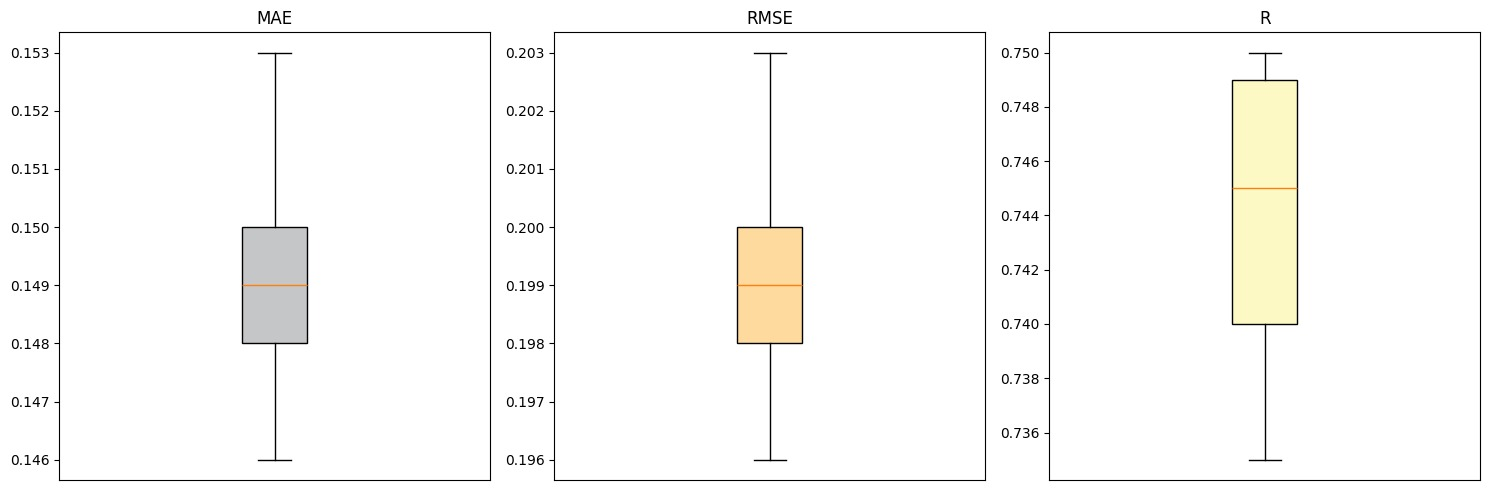
\includegraphics[width=1\linewidth]{2_CAPITULO5/IMG/box.jpeg}
                \begin{justify}
                    \textit{Nota.} Diagrama de cajas que muestra la variabilidad y dispersión de MAE, RMSE y coeficiente de Pearson en superresolución de imágenes MSS.
                \end{justify}                    
                \label{modelo}
            \end{figure}


            El diagrama de cajas proporciona una visión clara de la distribución estadística de las métricas de validación aplicadas a la superresolución de imágenes MSS en Perú. Cada métrica revela aspectos distintos de la precisión del modelo MSS2TM. El MAE destaca la exactitud media en la estimación de valores de píxeles, el RMSE señala la dispersión general de los errores en las predicciones del modelo, y el coeficiente de Pearson mide la fuerza y la dirección de la relación lineal entre las imágenes generadas y las originales.

            Los valores promedio de MAE y RMSE a lo largo de todas las imágenes evaluadas fueron 0.150 y 0.200, respectivamente, lo que indica un buen rendimiento general del modelo en el contexto de la superresolución. Sin embargo, hubo variabilidad en el rendimiento entre diferentes áreas, como lo demuestra el rango de valores de MAE y RMSE. La imagen identificada como 00328 mostró un desempeño sobresaliente con el MAE más bajo y el coeficiente de correlación de Pearson más alto, mientras que la imagen 06008 presentó los valores más altos de MAE y RMSE, además de la correlación más baja, lo que sugiere que ciertas áreas pueden presentar desafíos específicos para el modelo.

            Este análisis detallado permite no solo verificar la capacidad del modelo para generar imágenes TM de alta fidelidad a partir de imágenes MSS, sino también identificar áreas donde el modelo puede requerir ajustes o entrenamiento adicional para manejar condiciones específicas del paisaje.


        \subsection{Análisis de las bandas SWIR y térmica}

            Uno de los hallazgos más intrigantes de este estudio es el comportamiento particular de las bandas SWIR y térmica en las métricas de validación. Como se observa en la Tabla \ref{valores_metricas2}, estas bandas presentan un MAE y RMSE notablemente superiores a las demás, acompañados de coeficientes de Pearson significativamente más bajos, incluso negativos en el caso de la banda SWIR2. 

            Esta discrepancia se debe principalmente a las características únicas de estas bandas en comparación con las bandas ópticas. Mientras que las bandas ópticas, como el rojo, verde, y NIR, reflejan la radiación solar, las bandas SWIR y térmica miden la radiación infrarroja emitida por los objetos, lo cual es altamente influenciado por la temperatura superficial terrestre y las condiciones ambientales.

            La sensibilidad de las bandas SWIR y térmica a la variabilidad de las condiciones ambientales, como la temperatura y la humedad, puede aumentar los errores de predicción cuando se utilizan modelos entrenados predominantemente en bandas ópticas. Este fenómeno es particularmente pronunciado en áreas con diversidad geográfica y climática como Perú, donde la variación de la temperatura superficial puede ser extrema debido a la topografía variada del país.

            La baja autocorrelación espectral de estas bandas también contribuye a la dificultad en su predicción. A diferencia de las bandas ópticas, donde la correlación entre bandas puede ser explotada para mejorar la precisión de la predicción, las bandas SWIR y térmica frecuentemente no muestran una correlación directa con otras bandas, lo que resulta en un desafío mayor para los algoritmos de superresolución que dependen de estas correlaciones para generar predicciones precisas.

            Este análisis refuerza la importancia de desarrollar estrategias específicas para la armonización y superresolución de las bandas SWIR y térmica, posiblemente a través de la integración de modelos que incorporen variables ambientales y terrestres que afectan directamente a las mediciones en estas bandas.

        
        
        
% % \Chapter{}
% % \chapter{PRESUPUESTO}
% %     \begin{table}[H]
% %         \caption{\doublespacing \\ \textit{Presupuesto detallado para el proyecto de investigación.}}
% %         \begin{spacing}{1.5}
% %             \fontsize{8pt}{10pt}\selectfont  
% %             \begin{tabularx}{\linewidth}{*{4}{P{4.5cm}}} 
% %                 \toprule
% %                 \multicolumn{4}{c}{\textbf{Presupuesto total (Montos aproximados en S/.)}} \\ 
% %                 \midrule
% %                 \textbf{Rubro} & \textbf{Costo unitario} & \textbf{Cantidad} & \textbf{Total} \\
% %                 \midrule
% %                 Equipos: & & & \\ 
% %                 Laptop & 3000 & 1 & 3000 \\ 
% %                 Disco duro de 1 Tbyte & 200 & 1 & 200 \\ 
% %                 Internet: & & & \\ 
% %                 Servicio de internet (12 meses) & 1400 & 1 & 1400 \\
% %                 Papelería y útiles: & & & \\
% %                 Materiales de escritorio & 150 & 1 & 150 \\ 
% %                 Impresiones & 800 & 1 & 800 \\ 
% %                 Software: & & & \\ 
% %                 QGIS, Python, R (gratuitos) & 0 & 1 & 0 \\ 
% %                 \midrule
% %                 Tiempo de investigación: & & & \\
% %                 Medio sueldo mínimo mensual & 512.5 & 12 & 6150 \\
% %                 \midrule
% %                 \textbf{Total General:} & & & \textbf{11700} \\
% %                 \bottomrule
% %             \end{tabularx}
% %         \end{spacing}
% %         \vspace{1\baselineskip}
% %         \textit{Nota.} El presupuesto incluye equipamiento, servicios, materiales y el costo estimado del tiempo del investigador basado en medio sueldo mínimo mensual, reflejando la dedicación parcial al proyecto durante un año. No incluye otros posibles gastos indirectos o costos de oportunidad.
% %         \label{Presupuesto}
% %     \end{table}

